\documentclass[landscape]{foils}

\usepackage{ae}
%\usepackage{hyperref}
%\usepackage{thumbpdf}
\usepackage{graphicx}
\usepackage{color}
\usepackage[left=1cm,right=1cm,top=2cm,bottom=2cm]{geometry}
\usepackage{ragged2e}
\usepackage{amstext}
\usepackage{xspace}
\usepackage{fancyvrb}
\usepackage{amsmath}
\usepackage{url}
\usepackage{tabularx}
\usepackage{pause}

\newcommand{\stitle}[1]{{\centering\color{blue}\Large #1\par\vspace*{10pt}\hrule}}
\newcommand{\cstitle}[1]{{\centering\color{blue}\Large #1\par\vspace*{10pt}\hrule}}

\setlength{\columnsep}{0.5cm}
\setlength{\columnseprule}{0.4pt}

\renewcommand{\emph}[1]{\textcolor{red}{\bf #1}}

\newcommand{\igraph}{\texttt{{igraph}}\xspace}

\DefineVerbatimEnvironment{Myverb}{Verbatim}
{numbers=left,numbersep=5mm,frame=lines,fontsize=\small}

\newenvironment{narrow}[2]{%
  \begin{list}{}{%
      \setlength{\topsep}{0pt}%
      \setlength{\leftmargin}{#1}%
      \setlength{\rightmargin}{#2}%
      \setlength{\listparindent}{\parindent}%
      \setlength{\itemindent}{\parindent}%
      \setlength{\parsep}{\parskip}}%
    \item[]}{\end{list}}

\newcommand{\bull}{$\bullet$\xspace}

\newcommand{\command}[1]{\textcolor{red}{#1}}
\newcommand{\comment}[1]{\textcolor{blue}{#1}}

\begin{document}

\RaggedRight
% \color{white}
% \pagecolor{black}
\fvset{fontsize=\small}
\fvset{commandchars=\\\{\}}
\definecolor{grey}{gray}{0.75}
\fvset{frame=single, numbers=left, rulecolor=\color{grey}}

\MyLogo{\color{black}igraph -- a package for network analysis}

\thispagestyle{empty}
\vspace*{1cm}
{\centering
\hrule
\Large
\vspace*{1cm}
{\bf \textcolor{red}{igraph} -- a package for network analysis}
\vspace*{1cm}
\par
\hrule
\par
\vspace*{4cm}
\normalsize\textcolor{blue}{G\'abor Cs\'ardi}\\
\small \textcolor{blue}{\texttt{Gabor.Csardi@unil.ch}}
\par
\vspace*{1.5cm}
Department of Medical Genetics, \\
University of Lausanne, Lausanne, Switzerland\\
}

\newpage

\stitle{Outline}

% Outline:
\begin{enumerate}
\centering\Large
\vfill
\item Why another graph package?\\
\vfill
\item igraph architecture, data model and data representation\\
\vfill
\item Manipulating graphs\\
\vfill
\item Features and their time complexity\\
\vfill
\mbox{}
\vfill
\end{enumerate}

\newpage
\stitle{Why another graph package?}
\begin{itemize}
\item \texttt{graph} is slow. \texttt{RBGL} is slow, too.
\marginpar{\vspace*{3.5cm}}
\marginpar{\hspace*{-8cm}\includegraphics{transitivity}}
\begin{Myverb}
> \command{ba2}\comment{                                # graph \& RBGL}
\slshape A graphNEL graph with undirected edges
\slshape Number of Nodes = 100000 
\slshape Number of Edges = 199801  \pause
> \command{system.time(RBGL::transitivity(ba2))}
\slshape    user  system elapsed 
\slshape   7.517   0.000   7.567 \pause
> \command{summary(ba)}\comment{                        # igraph}
\slshape Vertices: 1e+05 
\slshape Edges: 199801 
\slshape Directed: FALSE 
\slshape No graph attributes.
\slshape No vertex attributes.
\slshape No edge attributes. \pause
> \command{system.time(igraph::transitivity(ba))}
\slshape    user  system elapsed 
\slshape   0.328   0.000   0.335 
\end{Myverb}
\end{itemize}

\newpage
\stitle{Why another graph package?}
\begin{itemize}
\item \texttt{sna} is slow. \texttt{network} is slow, too.
\begin{Myverb}
> \command{net2}\comment{                                  # SNA \& network}
\slshape  Network attributes:
\slshape   vertices = 1e+05 
\slshape   directed = TRUE 
\slshape   hyper = FALSE 
\slshape   loops = FALSE 
\slshape   multiple = FALSE 
\slshape   bipartite = FALSE 
\slshape   total edges= 199801 
\slshape     missing edges= 0 
\slshape     non-missing edges= 199801 
\slshape ... \pause
> \command{gtrans(net2)}
\slshape Error in matrix(0, nr = network.size(x), nc = network.size(x)) : 
\slshape   too many elements specified
\end{Myverb}
\end{itemize}

\newpage
\stitle{Why another graph package?}
\begin{itemize}
\item \texttt{graph} is slow. \texttt{RBGL} is slow, too.
\item \texttt{sna} is slow. \texttt{network} is slow, too.
\item A generic solution was needed, i.e. a common C layer, that 
  can be interfaced from C/C++, R, Python, etc.
\end{itemize} \pause
\begin{center}
\includegraphics[width=0.8\textwidth]{schema}
\end{center}

\newpage
\stitle{The igraph architecture}
\begin{center}
\vspace*{-2cm}
\includegraphics[width=0.8\textwidth]{arch}
\end{center}

\newpage
\stitle{Dependencies}
\begin{itemize}
% TODO: better look, e.g. add logos
\item Standard C/C++ libraries. 
  \marginpar{\vspace*{-1.5cm}}
  \marginpar{\hspace*{-6.5cm}%
    \includegraphics[width=3cm]{source_c}%
    \includegraphics[width=3cm]{source_cpp}%
%    \includegraphics[width=3cm]{gccegg-65}%
  }\\[-10pt]\pause
\item \texttt{stats} package, this is part of \texttt{base}.
  \marginpar{\vspace*{0.3cm}}
  \marginpar{\hspace*{-4cm}\mbox{ }%
    \includegraphics[width=3cm]{Rlogo-2}}\\[-10pt]\pause
\item Optional: \texttt{libxml2} library, for reading \\ GraphML files
  (included in Windows builds).
  \marginpar{\vspace*{-2.3cm}}
  \marginpar{\hspace*{-8.5cm}%
    \includegraphics[width=4.5cm]{Libxml2-Logo-180x168}
  }\\[-10pt]\pause
\item Optional: GMP library, graph automorphisms\\
  (not included in Windows builds). 
  \marginpar{\vspace*{-1.5cm}}
  \marginpar{\hspace*{-6cm}%
    \includegraphics[width=5.5cm]{gmplogo2}
  }\\[-10pt]\pause
\item Suggested packages: \texttt{stats4}, \texttt{rgl}, 
  \texttt{tcltk}, \texttt{RSQLite},\\
  \texttt{digest}, \texttt{graph},
  \texttt{Matrix}.\\
\begin{flushright}
\includegraphics[width=3cm]{Rlogo-2}
\includegraphics[width=3cm]{hist3d_2lights}
\includegraphics[width=2cm]{logo125}
\includegraphics[width=4cm]{SQLite}
\includegraphics[width=2cm]{hash_small}
\includegraphics[width=3cm]{plot}
\includegraphics[width=3cm]{matrix}
\end{flushright}
\end{itemize}

\newpage
\stitle{The igraph data model, what cannot be represented}

\begin{minipage}{0.6\textwidth}
  ``Mixed'' graphs, with undirected and directed edges.
  You can ``emulate'' them via graph attributes.
\end{minipage}\begin{minipage}{0.3\textwidth}
  \includegraphics[height=0.65\textwidth]{mixed}
\end{minipage} \par \pause
\vspace*{-1cm}
{\raggedleft
\begin{minipage}{0.3\textwidth}
  \raggedleft
  \includegraphics[height=0.65\textwidth]{hyper}
\end{minipage}\begin{minipage}{0.6\textwidth}
  Hypergraphs. Perhaps see the \texttt{hypergraph} package.
\end{minipage} \par
} \pause
\begin{minipage}{0.6\textwidth}
No direct support for bipartite (two-mode) graphs.\\
  It is possible to handle them via graph attributes.
\end{minipage}\begin{minipage}{0.3\textwidth}
  \includegraphics[height=0.65\textwidth]{bipartite}
\end{minipage}

\newpage
\stitle{Graph representation, sparse graphs}

Flat data structures, indexed edge lists. Easy to
handle, good for many kind of questions.
\begin{center}
  \includegraphics[width=0.55\textwidth]{igraph0}
\end{center}

\newpage
\stitle{Graph representation, sparse graphs}

Flat data structures, indexed edge lists. Easy to
handle, good for many kind of questions.
\begin{center}
  \includegraphics[width=0.55\textwidth]{igraph1}
\end{center}

\newpage
\stitle{Graph representation, sparse graphs}

Flat data structures, indexed edge lists. Easy to
handle, good for many kind of questions.
\begin{center}
  \includegraphics[width=0.55\textwidth]{igraph11}
\end{center}

\newpage
\stitle{Graph representation, sparse graphs}

Flat data structures, indexed edge lists. Easy to
handle, good for many kind of questions.
\begin{center}
  
\includegraphics[width=0.55\textwidth]{igraph2}
\end{center}

\newpage
\stitle{Graph representation, sparse graphs}

Flat data structures, indexed edge lists. Easy to
handle, good for many kind of questions.
\begin{center}
  
\includegraphics[width=0.55\textwidth]{igraph3}
\end{center}

\newpage
\stitle{Graph representation, sparse graphs}

Flat data structures, indexed edge lists. Easy to
handle, good for many kind of questions.
\begin{center}
  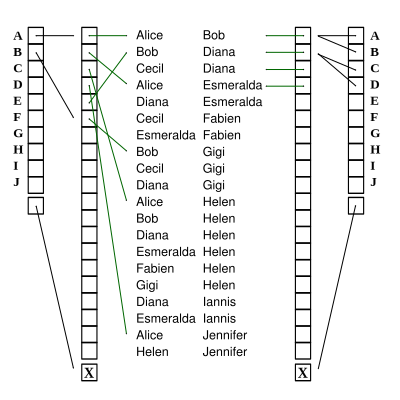
\includegraphics[width=0.55\textwidth]{igraph}
\end{center}

% \newpage
% \stitle{Vertex and edge ids}

\newpage
\stitle{Creating graphs, via vertex ids}
% TODO: plot
\begin{Myverb}
> \command{g <- graph( c(0,1, 1,2, 2,3, 3,4), n=6, directed=TRUE )}
> \command{g}
\slshape Vertices: 6 
\slshape Edges: 4 
\slshape Directed: TRUE 
\slshape Edges:
          
\slshape [0] 0 -> 1
\slshape [1] 1 -> 2
\slshape [2] 2 -> 3
\slshape [3] 3 -> 4
\end{Myverb}
\begin{flushright}
\vspace*{-6cm}
\includegraphics[width=0.45\textwidth]{g1}
\end{flushright}

\newpage
\stitle{Creating graphs, via vertex ids}
\begin{Myverb}
> \command{el <- cbind(0:9, 9:0)}
> \command{g <- graph( t(el), directed=TRUE)}
> \command{g}
\slshape Vertices: 10 
\slshape Edges: 10 
\slshape Directed: TRUE 
\slshape Edges:
          
\slshape [0] 0 -> 9
\slshape [1] 1 -> 8
\slshape [2] 2 -> 7
\slshape [3] 3 -> 6
\slshape [4] 4 -> 5
\slshape [5] 5 -> 4
\slshape [6] 6 -> 3
\slshape [7] 7 -> 2
\slshape [8] 8 -> 1
\slshape [9] 9 -> 0
\end{Myverb}
\begin{flushright}
\vspace*{-11.5cm}
\includegraphics[width=0.45\textwidth]{g2}
\end{flushright}

\newpage
\stitle{Creating graphs, \texttt{graph.formula}}
\begin{Myverb}
\comment{# A simple undirected graph}
> \command{g <- graph.formula( Alice-Bob-Cecil-Alice, }
\command{       Daniel-Cecil-Eugene, Cecil-Gordon )}
> \command{g}
\slshape Vertices: 6 
\slshape Edges: 6 
\slshape Directed: FALSE 
\slshape Edges:
                    
\slshape [0] Alice  -- Bob   
\slshape [1] Bob    -- Cecil 
\slshape [2] Alice  -- Cecil 
\slshape [3] Cecil  -- Daniel
\slshape [4] Cecil  -- Eugene
\slshape [5] Cecil  -- Gordon
\end{Myverb}
\begin{flushright}
\vspace*{-9.5cm}
\includegraphics[width=0.45\textwidth]{g3}
\end{flushright}

\newpage
\stitle{Creating graphs, \texttt{graph.formula}}
\begin{Myverb}
\comment{# Another undirected graph, ":" notation}
> \command{g2 <- graph.formula( Alice-Bob:Cecil:Daniel, }
\command{        Cecil:Daniel-Eugene:Gordon )}
> \command{g2}
\slshape Vertices: 6 
\slshape Edges: 7 
\slshape Directed: FALSE 
\slshape Edges:
                    
\slshape [0] Alice  -- Bob   
\slshape [1] Alice  -- Cecil 
\slshape [2] Alice  -- Daniel
\slshape [3] Cecil  -- Eugene
\slshape [4] Cecil  -- Gordon
\slshape [5] Daniel -- Eugene
\slshape [6] Daniel -- Gordon
\end{Myverb}
\begin{flushright}
\vspace*{-10.5cm}
\includegraphics[width=0.45\textwidth]{g4}
\end{flushright}

\newpage
\stitle{Creating graphs, \texttt{graph.formula}}
\begin{Myverb}
\comment{# A directed graph}
> \command{g3 <- graph.formula( Alice +-+ Bob --+ Cecil }
\command{        +-- Daniel, Eugene --+ Gordon:Helen )}
> \command{g3}
\slshape Vertices: 7 
\slshape Edges: 6 
\slshape Directed: TRUE 
\slshape Edges:
                    
\slshape [0] Bob    -> Alice 
\slshape [1] Alice  -> Bob   
\slshape [2] Bob    -> Cecil 
\slshape [3] Daniel -> Cecil 
\slshape [4] Eugene -> Gordon
\slshape [5] Eugene -> Helen 
\end{Myverb}
\begin{flushright}
\vspace*{-9.5cm}
\includegraphics[width=0.45\textwidth]{g5}
\end{flushright}

\newpage
\stitle{Creating graphs, \texttt{graph.formula}}
\begin{Myverb}
\comment{# A graph with isolate vertices}
> \command{g4 <- graph.formula( Alice -- Bob -- Daniel, }
\command{        Cecil:Gordon, Helen )}
> \command{g4}
\slshape Vertices: 6 
\slshape Edges: 2 
\slshape Directed: FALSE 
\slshape Edges:
                    
\slshape [0] Alice  -- Bob   
\slshape [1] Bob    -- Daniel
> \command{V(g4)}
\slshape Vertex sequence:
\slshape [1] "Alice"  "Bob"    "Daniel" 
\slshape [4] "Cecil"  "Gordon" "Helen"
\end{Myverb}
\begin{flushright}
\vspace*{-9.5cm}
\includegraphics[width=0.45\textwidth]{g6}
\end{flushright}

\newpage
\stitle{Creating graphs, \texttt{graph.formula}}
\begin{Myverb}
\comment{# "Arrows" can be arbitrarily long}
> \command{g5 <- graph.formula( Alice +---------+ Bob )}
> \command{g5}
\slshape Vertices: 2 
\slshape Edges: 2 
\slshape Directed: TRUE 
\slshape Edges:
                  
\slshape [0] Bob   -> Alice
\slshape [1] Alice -> Bob  
\end{Myverb}
\begin{flushright}
\vspace*{-5.5cm}
\includegraphics[width=0.45\textwidth]{g7}
\end{flushright}

\newpage
\stitle{Creating graphs, \texttt{graph.famous}}
\begin{Myverb}
> \command{graph.famous("Cubical")}
\slshape Vertices: 8 
\slshape Edges: 12 
\slshape Directed: FALSE 
\slshape Edges:
           
\slshape [0]  0 -- 1
\slshape [1]  1 -- 2
\slshape [2]  2 -- 3
\slshape [3]  0 -- 3
\slshape [4]  4 -- 5
\slshape [5]  5 -- 6
\slshape [6]  6 -- 7
\slshape [7]  4 -- 7
\slshape [8]  0 -- 4
\slshape [9]  1 -- 5
\slshape [10] 2 -- 6
\slshape [11] 3 -- 7
\end{Myverb}
\begin{flushright}
\vspace*{-11.5cm}
\includegraphics[width=0.45\textwidth]{g8}
\end{flushright}

\newpage
\stitle{Creating graphs, \texttt{graph.data.frame}}
\begin{Myverb}
> \command{traits <- read.csv("traits.csv", head=F)}
> \command{traits}
\slshape                   V1 V2 V3
\slshape 1     Alice Anderson 48  F
\slshape 2       Bob Bradford 33  M
\slshape 3       Cecil Connor 45  F
\slshape 4      David Daugher 34  M
\slshape 5  Esmeralda Escobar 21  F
\slshape 6       Frank Finley 36  M
\slshape 7         Gabi Garbo 44  F
\slshape 8         Helen Hunt 40  F
\slshape 9        Iris Irving 25  F
\slshape 10       James Jones 47  M
> \command{colnames(traits) <- c("name", "age", "gender")}
> \command{traits[,1] <- sapply(strsplit(as.character(traits[,1]), " "), "[", 1)}
\end{Myverb}

\newpage
\stitle{Creating graphs, \texttt{graph.data.frame}}
\begin{Myverb}
> \command{relations <- read.csv("relations.csv", head=F)}
> \command{relations}
\slshape           V1        V2 V3 V4 V5
\slshape 1        Bob     Alice  N  4  4
\slshape 2      Cecil       Bob  N  5  5
\slshape 3      Cecil     Alice  Y  5  5
\slshape 4      David     Alice  N  3  4
\slshape 5      David       Bob  N  4  2
\slshape 6  Esmeralda     Alice  Y  4  3
\slshape 7      Frank     Alice  N  3  2
\slshape 8      Frank Esmeralda  N  4  4
\slshape 9       Gabi       Bob  Y  5  5
\slshape 10      Gabi     Alice  N  3  0
\slshape 11     Helen     Alice  N  4  1
\slshape 12      Iris     Cecil  N  0  1
\slshape ...
> \command{colnames(relations) <- c("from", "to", "same.room", }
\command{          "friendship", "advice")}
\end{Myverb}

\newpage
\stitle{Creating graphs, \texttt{graph.data.frame}}
\begin{Myverb}
> \command{orgnet <- graph.data.frame(relations, vertices=traits)}
> \command{summary(orgnet)}
\slshape Vertices: 10 
\slshape Edges: 34 
\slshape Directed: TRUE 
\slshape No graph attributes.
\slshape Vertex attributes: name, age, gender.
\slshape Edge attributes: same.room, friendship, advice.
\end{Myverb}

\newpage
\stitle{Creating graphs, \texttt{graph.data.frame}}
\begin{Myverb}
> \command{plot(orgnet, layout=layout.kamada.kawai, vertex.label=V(orgnet)$name, }
\command{    vertex.shape="rectangle", vertex.size=20, asp=FALSE)}
\end{Myverb}
 % $
\begin{center}
\vspace*{-2cm}
\includegraphics[width=0.8\textwidth]{orgnet}
\end{center}

\newpage
\stitle{Creating graphs, random graphs}
\begin{Myverb}
> \command{er <- erdos.renyi.game(100, 100, type="gnm")}
> \command{plot(er, vertex.size=5, vertex.label=NA, asp=FALSE, vertex.shape="square",}
\command{       layout=layout.fruchterman.reingold, edge.color="black")}
\end{Myverb}
\begin{center}
\vspace*{-1cm}
\enlargethispage{2cm}
\includegraphics[width=0.75\textwidth]{er}
\end{center}

\newpage
\stitle{Creating graphs, random graphs}
\begin{Myverb}
> \command{ba <- ba.game(100, power=1, m=1)}
> \command{plot(ba, vertex.size=3, vertex.label=NA, asp=FALSE, vertex.shape="square",}
\command{       layout=layout.fruchterman.reingold, edge.color="black", }
\command{       edge.arrow.size=0.5)}
\end{Myverb}
\begin{center}
\vspace*{-1cm}
\enlargethispage{2cm}
\includegraphics[width=0.75\textwidth]{ba}
\end{center}

\newpage
\stitle{Meta data: graph/vertex/edge attributes}
\begin{itemize}
\item Assigning attributes:
  \texttt{set/get.graph/vertex/edge.attribute}. \pause
\item \verb+V(g)+ and \verb+E(g)+. \pause
\item Easy access of attributes:
  \begin{Myverb}
> \command{g <- erdos.renyi.game(30, 2/30)}
> \command{V(g)$color <- sample( c("red", "black"), }
\command{                        vcount(g), rep=TRUE)}
> \command{V(g)$color}
\slshape  [1] "red"   "black" "red"   "black" "black" "black" "red"   "red"   "red"  
\slshape [10] "black" "black" "black" "red"   "red"   "black" "red"   "black" "black"
\slshape [19] "red"   "red"   "black" "black" "red"   "black" "black" "red"   "black"
\slshape [28] "black" "black" "red"  
> \command{E(g)$color <- "grey"}
\end{Myverb}
% $
\end{itemize}

\newpage
\stitle{Vertex/edge selection with attributes}
\begin{Myverb}
> \command{red <- V(g)[ color == "red" ]}
> \command{bl <- V(g)[ color == "black" ]}
> \command{E(g)[ red %--% red ]$color <- "red"}
> \command{E(g)[ bl  %--% bl ]$color <- "black"}
> \command{plot(g, vertex.size=5, }
\command{       layout=layout.fruchterman.reingold, }
\command{       vertex.label=NA)}
\end{Myverb}
\vspace*{-5cm}
\begin{flushright}
\includegraphics[width=0.45\textwidth]{attr}
\end{flushright}

\newpage
\stitle{Visualizing graphs}
\begin{itemize}
\item Three functions with (almost) identical interfaces. \pause
\item \verb+plot+ Uses traditional R graphics, non-interactive, 2d.
  Publication quality plots in all formats R supports.
\begin{Myverb}
> \command{g <- barabasi.game(100, m=1)}
> \command{igraph.par("plot.layout", }
\command{             layout.fruchterman.reingold)}
> \command{plot(g, vertex.size=4, vertex.label=NA, }
\command{       edge.arrow.size=0.7, }
\command{       edge.color="black",}
\command{       vertex.color="red", frame=TRUE)}
\end{Myverb}
\end{itemize}
\begin{flushright}
\vspace*{-8cm}
\includegraphics[width=0.45\textwidth]{plot}
\end{flushright}

\newpage
\stitle{Visualizing graphs}
\verb+tkplot+ Uses Tcl/Tk via the \verb+tcltk+ package, 
  interactive, 2d.
\begin{Myverb}
> \command{id <- tkplot(g, vertex.size=4, }
\command{        vertex.label=NA,}
\command{        edge.color="black",}
\command{        edge.arrow.size=0.7,}
\command{        vertex.color="red")}
> \command{coords <- tkplot.getcoords(id)}
\end{Myverb}
\begin{flushright}
\vspace*{-6cm}
\includegraphics{tkplot}
\end{flushright}

\newpage
\stitle{Visualizing graphs}
\verb+rglplot+ Needs the \verb+rgl+ package.
\begin{Myverb}
> \command{co <- layout.kamada.kawai(g, dim=3)}
> \command{rglplot(g, vertex.size=5, }
\command{           vertex.label=NA, }
\command{           layout=co)}
\end{Myverb}
\begin{flushright}
\vspace*{-6cm}
\enlargethispage{3cm}
\includegraphics{rglplot}
\end{flushright}

\newpage
\stitle{Working with a somewhat bigger graph}
\begin{Myverb}
> \command{vertices <- read.csv("http://cneurocvs.rmki.kfki.hu/igraph/judicial.csv")}
> \command{edges <- read.table("http://cneurocvs.rmki.kfki.hu/igraph/allcites.txt")}
> \command{jg <- graph.data.frame(edges, vertices=vertices, dir=TRUE)}
> \command{summary(jg)}
\slshape Vertices: 30288 
\slshape Edges: 216738 
\slshape Directed: TRUE 
\slshape No graph attributes.
\slshape Vertex attributes: name, usid, parties, year, overruled, overruling,
\slshape   oxford, liihc, indeg, outdeg, hub, hubrank, auth, authrank, between, incent.
\slshape No edge attributes.
\end{Myverb}

\newpage
\stitle{Working with a somewhat bigger graph}
\begin{Myverb}
> \command{is.connected(jg)}\comment{                   # Is it connected?}
\slshape [1] FALSE\pause

> \command{no.clusters(jg)}\comment{                    # How many components?}
\slshape [1] 4881\pause

> \command{table(clusters(jg)$csize)}\comment{          # How big are these?}

\slshape     1     3     4 25389 
\slshape  4871     8     1     1 \pause

> \command{max(degree(jg, mode="in"))}\comment{         # Vertex degree}
\slshape [1] 248
> \command{max(degree(jg, mode="out"))}
\slshape [1] 195
> \command{max(degree(jg, mode="all"))}
\slshape [1] 313
\end{Myverb}
%$

\newpage
\stitle{Working with a somewhat bigger graph}
\begin{Myverb}
\comment{# In-degree distribution}
> \command{plot(degree.distribution(jg, mode="in"), log="xy")}
\end{Myverb}
\begin{center}
\includegraphics[width=0.7\textwidth]{indd}
\end{center}

\newpage
\stitle{Working with a somewhat bigger graph}
\begin{Myverb}
\comment{# Out-degree distribution}
\command{plot(degree.distribution(jg, mode="out"), log="xy")}
\end{Myverb}
\begin{center}
\includegraphics[width=0.7\textwidth]{outdd}
\end{center}

\newpage
\stitle{Working with a somewhat bigger graph}
\begin{Myverb}
\comment{# Taking the largest component}
> \command{cl <- clusters(jg)}
> \command{jg2 <- subgraph(jg, which(cl$membership == which.max(cl$csize)-1)-1)}
> \command{summary(jg2)}
\slshape Vertices: 25389 
\slshape Edges: 216718 
\slshape Directed: TRUE 
\slshape No graph attributes.
\slshape Vertex attributes: name, usid, parties, year, overruled, overruling, 
\slshape    oxford, liihc, indeg, outdeg, hub, hubrank, auth, authrank, 
\slshape    between, incent.
\slshape No edge attributes.
\end{Myverb}

\newpage
\stitle{Working with a somewhat bigger graph}
\begin{Myverb}
> \command{graph.density(jg2)}\comment{                        # Density}
\slshape [1] 0.0003362180\pause

> \command{transitivity(jg2)}\comment{                         # Transitivity}
\slshape [1] 0.1260031\pause

\comment{# Transitivity of a random graph of the same size}
> \command{g <- erdos.renyi.game(vcount(jg2), ecount(jg2), type="gnm")}
> \command{transitivity(g)}
\slshape [1] 0.00064649\pause

\comment{# Transitivity of a random graph with the same degrees}
> \command{g2 <- degree.sequence.game(degree(jg2,mode="all"), method="vl")}
> \command{transitivity(g2)}
\slshape [1] 0.004107072
\end{Myverb}

\newpage
\stitle{Community structure detection}
\begin{Myverb}
> \command{fc <- fastgreedy.community(simplify(as.undirected(jg2)))}
> \command{memb <- community.to.membership(jg2, }
\command{          fc$merges,}
\command{          which.max(fc$modularity)) }
> \command{lay <- layout.drl(jg2)}
> \command{jg3 <- graph.empty(n=vcount(jg2))}
> \command{colbar <- rainbow(5)}
> \command{col <- colbar[memb$membership+1] }
> \command{col[is.na(col)] <- "grey"}
> \command{plot(jg3, layout=lay, vertex.size=1, }
\command{       vertex.label=NA, asp=FALSE,}
\command{       vertex.color=col, }
\command{       vertex.frame.color=col)}
\end{Myverb}
%$
\begin{flushright}
\vspace*{-9.5cm}
\includegraphics{jgplot}
\end{flushright}

\newpage
\stitle{Functionality, what can be calculated?}
\renewcommand{\arraystretch}{1.7}
\begin{tabularx}{\textwidth}{l|X}
Fast (millions) & creating graphs (most of the time) \bull
       structural modification (add/delete edges/vertices) \bull 
       subgraph \bull simplify \bull graph.decompose \bull 
       degree \bull clusters \bull graph.density \bull is.simple,
       is.loop, is.multiple \bull articulation points and biconnected
       components \bull ARPACK stuff: page.rank, hub.score,
       authority.score, eigenvector centrality \bull transitivity \bull Burt's
       constraint \bull dyad \& triad census, graph motifs \bull
       $k$-cores \bull MST \bull reciprocity \bull modularity \bull
       closeness and (edge) betweenness \it{estimation} \bull shortest
       paths from one source \bull generating $G_{n,p}$ and $G_{n,m}$
       graphs \bull generating PA graphs with various PA exponents
       \bull topological sort \\
\hline
Slow (10000) & closeness \bull diameter \bull betweenness \bull all-pairs
       shortest paths, average path length \bull most layout
       generators \bull \\
\hline
Very slow (100) & cliques \bull cohesive blocks \bull edge/vertex
            connectivity \bull maximum flows and minimum cuts \bull 
            power centrality \bull alpha centrality \bull (sub)graph isomorphism\\
\end{tabularx}

\newpage
\stitle{Connection to other network/graph software}
\begin{itemize}
\item \texttt{graph} package: \texttt{igraph.to.graphNEL},
  \texttt{igraph.from.graphNEL}. \pause
\item Sparse matrices (\texttt{Matrix} package),
  \texttt{get.adjacency} and \texttt{graph.adjacency} supports them. \pause
\item \texttt{sna} and \texttt{network} R packages. Currently throught
  adjacency matrices. Use namespaces! \pause
\item Pajek. \texttt{.net} file format is supported. \pause
\item Visone. Use GraphML format. \pause
\item Cytoscape. Use GML format. \pause
\item GraphViz. igraph can write \texttt{.dot} files. \pause
\item In general. The \texttt{GraphML} and \texttt{GML} file formats 
  are fully supported, many programs can read/write these.
\end{itemize}

\newpage
\stitle{Acknowledgements}
\begin{center}
\setlength{\parskip}{30pt}
\vfill
Tam\'as Nepusz\par\vfil
Peter McMahan, the BLISS, Walktrap, Spinglass, DrL projects\par\vfil
All the people who contributed code, sent bug reports, suggestions\par\vfil
The R project\par\vfil
\end{center}
\vfill\mbox{}\vfill

\end{document}
